\TieudeT{PHONG TỎA VẬT LÍ}
\subsubsection*{PHẦN I. Thí sinh trả lời câu hỏi từ câu 1 đến câu 18. Mỗi câu hỏi thí sinh chỉ chọn một phương án}
\setcounter{ex}{0}
\begin{ex}%book
Trong Vật lí, chất lưu dùng để chỉ
\choice
{chất lỏng}
{chất rắn}
{chất khí}
{\True chất lỏng và khí}
\loigiai{}
\haidong{10} \end{ex}
\begin{ex}%book
Lực cản của chất lưu tác dụng lên vật phụ thuộc vào yếu tố nào?
\choice
{chỉ phụ thuộc vào hình dạng của vật}
{chỉ phụ thuộc vào tốc độ của vật}
{\True phụ thuộc vào hình dạng và tốc độ của vật}
{không phụ thuộc vào tốc độ của vật}
\loigiai{Lực cản của chất lưu tác dụng lên vật phụ thuộc vào hình dạng và tốc độ của vật.}
\haidong{10} \end{ex}
\begin{ex}%book
Phát biểu nào sau đây là \textbf{sai}?
\choice
{Các chất lỏng khác nhau tác dụng lực cản khác nhau lên cùng một vật}
{Lực cản của nước muối lớn hơn lực cản của nước lọc}
{\True Các chất lỏng khác nhau tác dụng lực cản như nhau lên cùng một vật}
{Lực cản của nước lớn hơn lực cản của không khí}
\loigiai{}
\haidong{10} \end{ex}
\begin{ex}%book
Phát biểu nào sau đây là \textbf{sai}?
\choice
{\True Người đang bơi trong nước chịu cả lực cản của không khí và của nước}
{Người đi bộ trên mặt đất chịu lực cản của không khí}
{Xe ô tô đang chạy chịu lực cản của không khí}
{Máy bay đang bay chịu lực cản của không khí}
\loigiai{}
\haidong{10} \end{ex}
\begin{ex}%book
Trong các trường hợp sau, trường hợp nào chịu lực cản của không khí nhỏ nhất?
\choice
{Người đạp xe giữ lưng thẳng khi đi}
{Người đạp xe khum lưng khi đi}
{\True Người đạp xe cúi gập người xuống khi đi}
{Người đạp xe nghiêng người sang phải khi đi}
\loigiai{}
\haidong{10} \end{ex}
\begin{ex}%book
Lực cản \textbf{không} phụ thuộc vào yếu tố nào sau đây?
\choice
{Vận tốc của vật}
{Hình dạng của vật}
{\True Khối lượng của vật}
{Cả vận tốc và hình dạng của vật}
\loigiai{	}
\haidong{10} 
\end{ex}
\begin{ex}%book
Phát biểu nào sau đây là đúng?
\choice
{Độ lớn của lực cản càng lớn khi diện tích mặt cản càng nhỏ}
{\True Độ lớn của lực cản càng lớn khi diện tích mặt cản càng lớn}
{Vật đi càng nhanh thì lực cản của không khí càng nhỏ}
{Tờ giấy để phẳng rơi nhanh hơn hòn đá}
\loigiai{}
\haidong{10} \end{ex}
\begin{ex}%book
Khi vật nổi trên chất lỏng thì lực đẩy Archimedes
\choice
{bằng trọng lượng riêng của nước nhân với thể tích của vật}
{bằng trọng lượng vật}
{\True bằng trọng lượng của phần nước bị vật chiếm chỗ}
{bằng trọng lượng của phần vật chìm trong nước}
\loigiai{}
\haidong{10} \end{ex}
\begin{ex}%book%SBT CTST 11.9
Một vật đang lơ lửng ở trong nước chịu tác dụng của những lực nào?
\choice
{Lực đẩy Archimedes và lực cản của nước}
{Lực đẩy Archimedes và lực ma sát}
{Trọng lực và lực cản của nước}
{\True Trọng lực và lực đẩy Archimedes}
\haidong{10} 
\end{ex}
\begin{ex}%book
Khi móc một vật vào lực kế trong không khí thì lực kế chỉ 50 N. Nếu nhúng chìm vật đó vào trong nước, số chỉ lực kế sẽ
\choice
{tăng lên}
{\True giảm đi}
{không đổi}
{chỉ số $0$}
\loigiai{}
\haidong{10} \end{ex}
\begin{ex}%book
Một quả bóng bay có thể bay lên trên không khí. Giải thích nào sau đây là đúng?
\choice
{Trong bóng bay có bơm một loại khí và Trái đất không hút các loại khí}
{Do bóng bay nhẹ hơn không khí}
{\True Do trong bóng bay người ta bơm khí hiđro có khối lượng riêng rất nhỏ, khí hidrô này tác dụng lên quả bóng một lực nâng lớn hơn trọng lượng của quả bóng}
{Do trọng lượng của quả bóng lớn hơn trọng lực do Trái Đất tác dụng lên quả bóng}
\loigiai{}
\haidong{10} \end{ex}
\begin{ex}%book
Khi máy bay cất cánh, phần trước máy bay hướng chéo lên để
\choice
{lực nâng tăng dần, giúp cho máy bay hạ thấp độ cao}
{\True lực nâng tăng dần, giúp cho máy bay chuyển động lên cao hơn}
{lực nâng giảm dần, giúp cho máy bay hạ thấp độ cao}
{lực nâng giảm dần, giúp cho máy bay chuyển động lên cao hơn}
\loigiai{}
\haidong{10} \end{ex}
\begin{ex}%book
Một vật khối lượng $2,5\ kg$ rơi thẳng đứng từ độ cao $100\ m$ không vận tốc đầu, sau $20\ s$ thì chạm đất. Lực cản của không khí (coi như không đổi) tác dụng lên vật có độ lớn là
\choice
{\True $23,75\ N$}
{$40\ N$}
{$20\ N$}
{$25\ N$}
\haidong{6}
\loigiai{
Chọn trục tọa độ Oy gắn với quỹ đạo rơi của vật, gốc tọa độ tại mặt đất, chiều dương hướng xuống.
 Viết phương trình chuyển động của vật $\Rightarrow a=0,5\ m/s^2$

Áp dụng biểu thức định luật II Newton:

$P-Fc=ma \Rightarrow Fc=mg-ma=m(g-a)=2,5(10-0,5)=23,75\ N$

}
\haidong{10} 
\end{ex}
\begin{ex}%book%SBT KNTT 19.6
Một chiếc xe ô tô có khối lượng tổng cộng người và xe là $550\ kg$ đang chuyển động trên mặt đường nằm ngang. Biết lực đẩy gây ra bởi động cơ tác dụng lên ô tô là $300\ N$ và tổng lực cản của môi trường lên ô tô là $200\ N$. Gia tốc của ô tô là
\choice
{$1,80\ m/s^2$}
{$1,08\ m/s^2$}
{\True $0,18\ m/s^2$}
{$1,28\ m/s^2$}
\haidong{4}
\loigiai{
\begin{itemize}
\item $F=F_{\ct{đẩy}}-F_{\ct{cản}}=300-200=100\ N$
\item $a=\dfrac{F}{m}=\dfrac{100}{550}\approx 0,18\ m/s^2$.
\end{itemize}
}
\haidong{10} \end{ex}
\begin{ex}%book%SBT KNTT 19.7
Lực đẩy tối đa có thể tác dụng lên một chiếc xe thể thao để nó chuyển động trên mặt đường nằm ngang là $500\ N$. Biết lực cản của không khí tác dụng lên xe phụ thuộc vào vận tốc $v$ theo công thức $F=0,2v^2$. Tốc độ tối đa của xe là
\choice
{\True $50\ m/s$}
{$60\ m/s$}
{$70\ m/s$}
{$80\ m/s$}
\haidong{10} \end{ex}
\begin{ex}%book
Một chiếc ca nô nặng $1$ tấn đang chuyển động dọc theo một dòng sông. Lực đẩy của động cơ là $900\ N$, lực cản của nước có độ lớn là $150\ N$, lực cản của không khí có độ lớn là $50\ N$. Gia tốc của ca nô có độ lớn là
\choice
{$0,5\ m/s^2$}
{$0,6\ m/s^2$}
{\True $0,7\ m/s^2$}
{$0,8\ m/s^2$}
\haidong{7}
\loigiai{
Áp dụng định luật II Niwton cho vật ta có

$\vec{F}_{C K}+\vec{F}_{C N}+\vec{P}+\vec{F}+\vec{F}_{N}=m \vec{a}(1)$

Chiếu (1) lên chiều chuyển động $\square a=0,7\ m/s^2$

}
\haidong{10} \end{ex}
\begin{ex}%book%SBT KNTT 19.8
\immini[thm]{Hình bên biểu diễn các vectơ lực tác dụng lên một máy bay đang bay ngang ở độ cao ổn định với tốc độ không đổi. Lấy $g=10\ m/s^2$. Nếu khối lượng tổng cộng của máy bay là $77$ tấn thì lực nâng có độ lớn bằng	
\choice
{\True $77.10^4\ N$}
{$7,7.10^4\ N$}
{$77\ N$}
{$7,7\ N$}}{\begin{tikzpicture}
\node[] at (0,0){\begin{tikzpicture}
\node[] at (0,0){
\includegraphics[width=5cm]{images/19-6}};
\end{tikzpicture}};
\end{tikzpicture}}
\haidong{6}
\haidong{10} \end{ex}

\begin{ex}%book
Treo một vật ở ngoài không khí vào lực kế, lực kế chỉ $2,1\ N$. Nhúng chìm vật đó vào nước thì số chỉ của lực kế giảm $0,2\ N$. Biết trọng lượng riêng của nước là $10000\ N / m^3$. Chất làm vật đó có trọng lượng riêng lớn gấp bao nhiêu lần trọng lượng riêng của nước? 
\choice
{$6$}
{$10$}
{\True $10,5$}
{$8$}
\haidong{6}
\loigiai{
Khi nhúng chìm vật vào nước, vật chịu tác dụng của lực đẩy Ác-si-mét nên số chỉ của lực kế giảm $0,2\ N$ tức là $F_{A}=0,2\ N$.

\begin{itemize}
\item Ta có: $F_{A}=V d_{n}$
\end{itemize}

$
V=\dfrac{F_{A}}{d_{n}}=\dfrac{0,2}{1000}=0,0002\left(\ m^3\right); d=\dfrac{P}{V}=\dfrac{2,1}{0,0002}=105000\left(\ N / m^3\right) \Rightarrow \dfrac{d}{d_{n}}=10,5
$

}
\haidong{10} \end{ex}





\subsubsection*{PHẦN 2. Thí sinh trả lời từ câu 1 đến câu 4. Trong mỗi ý a), b), c), d) ở mỗi câu, thí sinh chọn đúng hoặc sai.}
\setcounter{ex}{0}
\begin{ex}%book
Lực cản là một khái niệm vật lý cơ bản, mô tả lực chống lại chuyển động của vật thể trong môi trường. Để kiểm tra sự hiểu biết của bạn về lực cản, hãy đánh giá phát biểu sau đây.
\choiceTF[t]
{Bạn Hoa chạy nhanh sẽ chịu lực cản ít hơn bạn Hoa chạy chậm}
{Đi xe máy chạy nhanh chịu lực cản ít hơn đi xe đạp chạy chậm}
{\True Lực cản của nước lớn hơn lực cản của không khí}
{Vật có hình dạng khí động học sẽ chịu lực cản lớn hơn}
\loigiai{}
\haidong{10} \end{ex}
\begin{ex}%book
Một vật có khối lượng riêng $2200\ kg/m^3$. Treo vật vào một lực kế rồi nhúng vật ngập trong nước thì lực kế chỉ $30\ N$. Lấy khối lượng riêng của nước là $1000\ kg/m^3$ và gia tốc trọng trường $g=10\ m/s^2$. 
\choiceTF[t]
{\True Số chỉ của lực kế khi để ngoài không khí chính là trọng lượng của vật}
{\True Khi nhúng vật vào trong nước thì vật chịu thêm lực đẩy Archimedes nên số chỉ của lực kế giảm xuống}
{Khi nằm cân bằng trong nước thì trọng lượng của vật bằng lực đẩy Archimede}
{\True Treo vật ở ngoài không khí thì lực kế chỉ $55\ N$}
\loigiai{\begin{itemchoice}
\itemch Đúng. Vì khối lượng riêng của không khí rất nhỏ (khoảng $1,29\ kg/m^3$ ) nên lực đẩy Archimedes tác dụng vào vật không đáng kể, có thể bỏ qua. Treo vật vào một lực kế thì vật chịu tác dụng của trọng lực và lực đàn hồi. Khi vật cân bằng thì độ lớn hai lực này bằng nhau. Vì vậy, số chỉ của lực kế khi để ngoài không khí chính là trọng lượng của vật.
\itemch Đúng. Khi nhúng vật vào trong nước thì vật chịu tác dụng thêm lực đẩy Archimedes hướng lên. Để vật cân bằng thì: $F_{d h}+F_{A}=P \Rightarrow F_{d h}=P-F_{A} \Rightarrow$ số chỉ của lực kế giảm xuống.
\itemch Sai. Khi nằm cân bằng trong nước thì: $F_{d h}+F_{A}=P$
\itemch Đúng. Khi nhúng vật vào trong nước thì lực đẩy Archimedes là: $F_{A}=V_{v} . \rho_{n} . g=\dfrac{m}{\rho_{v}} . \rho_{n} . g=\dfrac{\rho_{n}}{\rho_{v}} . P$\\
Khi vật cân bằng trong nước: $P-F_{A}=F_{d h} \Rightarrow P-\dfrac{\rho_{n}}{\rho_{v}} . P=F_{d h} \Rightarrow P=\dfrac{F_{d h}}{1-\dfrac{\rho_{n}}{\rho_{v}}}=\dfrac{30}{1-\dfrac{1000}{2200}}=55 \ N$
\end{itemchoice}
}

\haidong{15} \end{ex}
\begin{ex}%book
\immini[thm]{Một khối gỗ hình hộp chữ nhật có tiết diện $S=40\ cm^2$, cao $h=10 \ cm$. Có khối lượng $m=160 \ g$. Lấy $g=10\ m/s^2$ và khối lượng riêng của nước là $\rho=1000\ kg/m^3$. Thả khối gỗ vào nước, khối gỗ nổi lơ lửng trên mặt nước như hình vẽ.}{
\includegraphics[width=4cm]{images/khoigo22pbdep}}
\choiceTF[t]
{Lực đẩy Archimedes phụ thuộc vào trọng lượng riêng của vật và thể tích của phần chất lỏng bị vật chiếm chỗ}
{\True Khi khối gỗ cân bằng trong nước thì trọng lượng của khối gỗ cân bằng với lực đẩy Archimedes}
{\True Trọng lượng của khối gỗ là $1,6\ N$}
{Khi khối gỗ cân bằng trong nước thì chiều cao của phần gỗ nổi trên mặt nước là $4\ cm$}			
\loigiai{\begin{itemchoice}
\itemch Sai. Lực đẩy Archimedes phụ thuộc vào trọng lượng riêng của chất lỏng và thể tích của phần chất lỏng bị vật chiếm chỗ
\itemch Đúng. Khối gỗ chịu tác dụng của trọng lực $\overrightarrow{P}$ và lực đẩy Archimedes $\overrightarrow{F}_{\text {asm}}$ nên khi khối gỗ cân bằng trong nước thì 2 lực này cân bằng nhau.
\itemch Đúng. Trọng lượng của khối gỗ là $P=m g=0,16 . 10=1,6 \ N$
\itemch Sai. Gọi $x$ là chiều cao phần mà khối gỗ nổi trên mặt nước, khi đó chiều cao phần chìm trong nước là $h-x$.

Thể tích phần gỗ chìm trong nước chính bằng thể tích phần nước bị gỗ chiếm chỗ: $V=S(h-x)$

Ta có: $P=F_{A} \Rightarrow m g=\rho g V \Rightarrow m=\rho S(h-x) \Rightarrow x=h-\dfrac{m}{\rho S}=0,1-\dfrac{0,16}{1000 . 30 . 10^{-4}}=0,06 \ m=6 \ cm$
\end{itemchoice}
}
\haidong{15} \end{ex}
\begin{ex}%book%nguon Huong Dan On Thi Tot Nghiep THPT Nguyen Van Bien
\immini[thm]{Một cậu bé có khối lượng $38\ kg$ trượt xuống một máng trượt trong công viên nước. Máng trượt nghiêng so với phương ngang một góc $30^\circ$. Hình bên biểu diễn các lực tác dụng vào cậu bé trong quá trình trượt, gồm: trọng lực $\vec{P}$, lực ma sát trượt $\vec{F}_{ms}$ và phản lực máng $\vec{N}$. Biết $F_{ms}=100 \ N$. Lấy gia tốc rơi tự do là $g=9,8\ m/s^2$.}{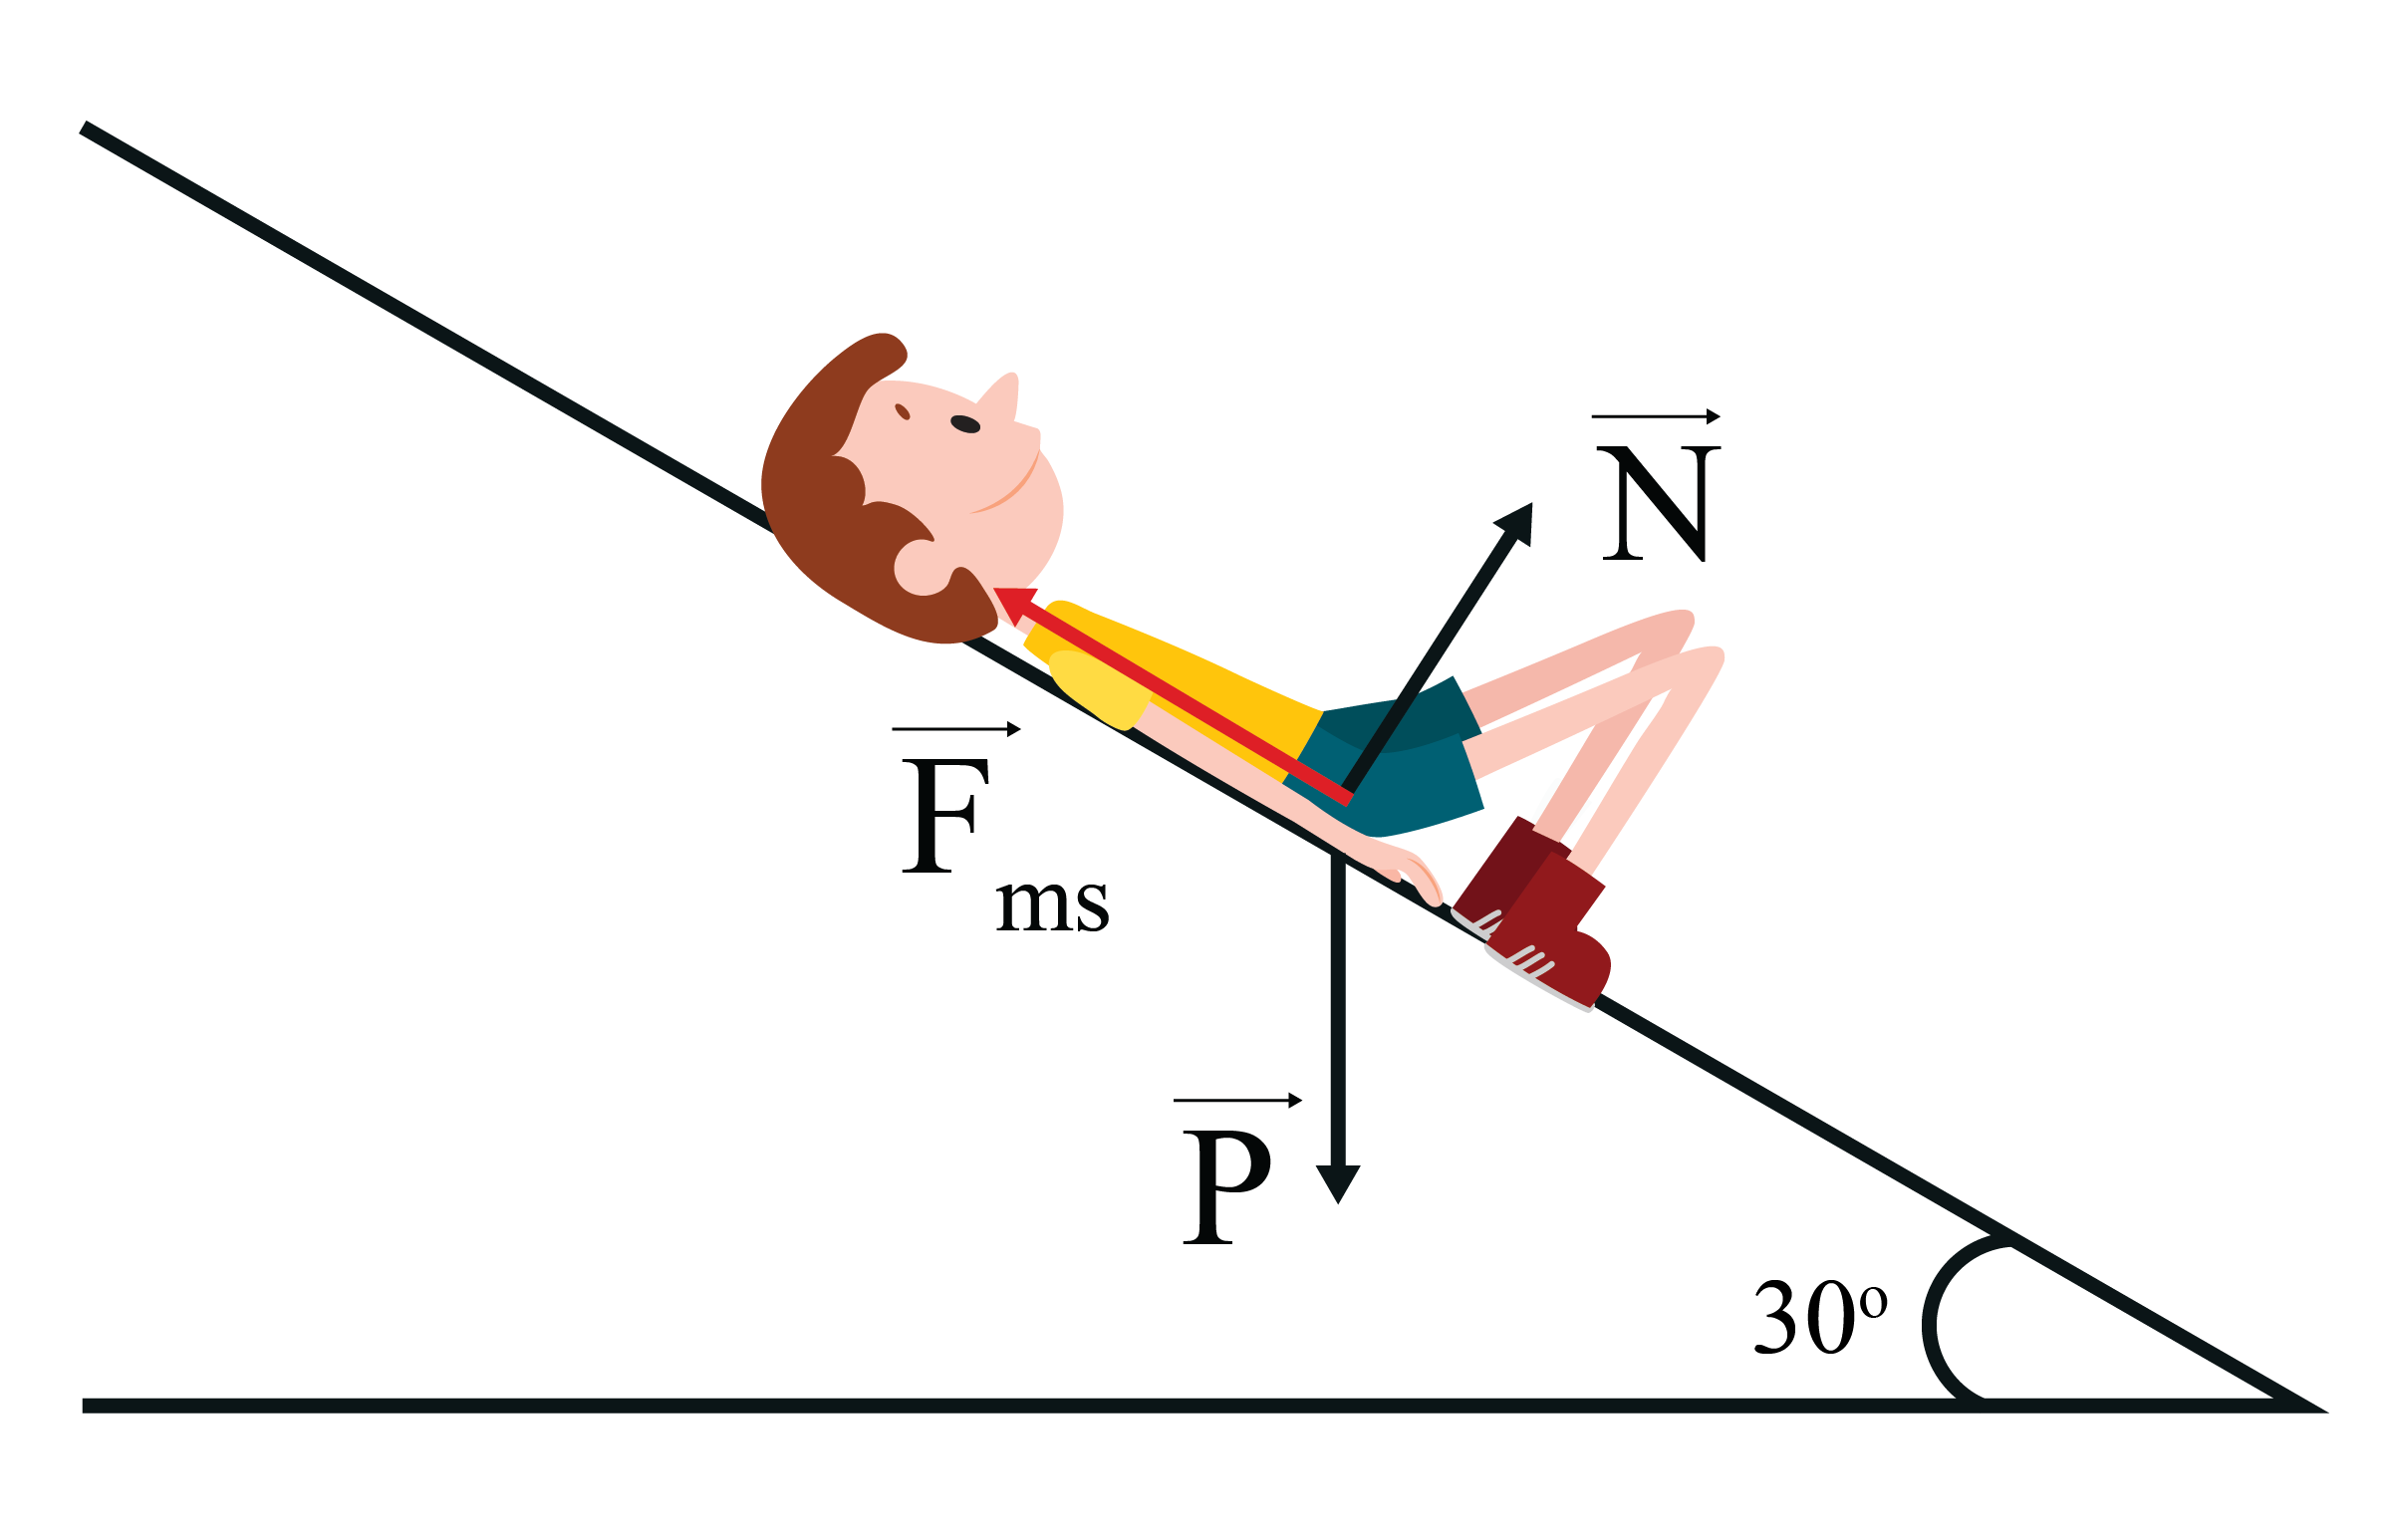
\includegraphics[width=4.5cm]{Images/caubetruotdep}}
\choiceTF[t]
{\True Trọng lượng của cậu bé là $372,4\ N$}
{Phản lực của máng trượt tác dụng lên cậu bé có độ lớn $186,2\ N$}
{\True Gia tốc của cậu bé có độ lớn xấp xỉ $2,3\ m/s^2$}
{Áp lực mà cậu bé tác dụng lên máng trượt nhỏ hơn lực ma sát trượt do máng tác dụng lên cậu bé}
\loigiai{
\begin{itemchoice}
\itemch
\itemch
\itemch
\itemch
\end{itemchoice}
}
\haidong{15} \end{ex}




















\subsubsection*{PHẦN 3. Thí sinh trả lời từ câu 1 đến câu 6.}
\setcounter{ex}{0} 
\textit{Sử dụng thông tin sau cho Câu 1 và Câu 2:} Một máy bay có khối lượng $10$ tấn đang bay ngang ở độ cao ổn định với tốc độ không đổi dưới tác dụng của lực đẩy của động cơ là $45000\ N$.
\begin{ex}
Lực nâng của không khí tác dụng lên máy bay là bao nhiêu kilô niutơn?
\shortans[oly]{100}
\loigiai{
Có 4 lực tác dụng lên máy bay:

\begin{itemize}
\item Lực đẩy của động cơ $\vec{F}$

\item Lực cản của không khí $\vec{F}_C$

\item Trọng lực $\vec{P}$

\item Lực nâng của không khí $\vec{F}_{N}$

\end{itemize}

Vì máy bay bay với độ cao ổn định và tốc độ không đổi nên:

$\vec{F}_C+\vec{F}_{N}+\vec{P}+\vec{F}=\overrightarrow{0}(1)$

Chiếu (1) lên phương thẳng đứng ta có: $F_{N}=P=m g=10000.10=100000\ N$
}
\end{ex}
\begin{ex}
Lực cản của không khí tác dụng lên máy bay là bao nhiêu kilô niutơn?
\shortans[oly]{45}
\loigiai{
Chiếu (1) lên phương ngang ta có: $F_C=F=m g=45000\ N$		
}
\haidong{10} \end{ex}



\textit{Sử dụng thông tin sau cho Câu 3 và Câu 4:} Một chiếc thuyền máy đang chuyển động dọc theo một dòng sông. Lực đẩy của máy thuyền là $500\ N$, lực ma sát giữa thuyền và nước là $100\ N$, lực cản của không khí lên thuyền là $50\ N$. Trọng lượng của thuyền là $2$ tấn.
\begin{ex}%book
Lực nâng của nước tác dụng lên thuyền là bao nhiêu kilô niutơn?
\shortans[oly]{20}
\end{ex}
\begin{ex}%book
Gia tốc chuyển động của thuyền là bao nhiêu $cm/s^2$?
\shortans[oly]{17,5}
\haidong{10}
\loigiai{
a) Có 4 lực tác dụng lên thuyền:

\begin{itemize}
\item Trọng lực $\vec{P}$

\item Lực đẩy của động cơ $\vec{F}$

\item Lực cản của không khí $\vec{F}_{C K}$

\item Lực cản của nước $\vec{F}_{C N}$

\item Lực nâng của nước $\vec{F}_{N}$

\end{itemize}

Áp dụng định luật II Niwton cho vật ta có

$\vec{F}_{C K}+\vec{F}_{C N}+\vec{P}+\vec{F}+\vec{F}_{N}=m \vec{a}(1)$

Chiếu (1) lên phương thẳng đứng ta có: $F_{N}=P=m g=2000.10=20000\ N$

b) Chiếu (1) lên phương ngang ta có:

$	F-F_{C K}-F_{C N}=m a
\Leftrightarrow 500-50-150=m a
\Rightarrow a=\dfrac{350}{2000}=0,175\ m/s^2	$

}
\haidong{10} \end{ex}
\textit{Sử dụng thông tin sau cho Câu 5 và Câu 6:} Một tảng băng có khối lượng riêng là $800 \ kg/m^3$ đang lơ lửng trên mặt nước biển. Khối lượng riêng của nước biển là $1020 \ kg/m^3$.
\begin{ex}%book
Tỉ lệ phần trăm phần thể tích của băng chìm dưới nước là bao nhiêu $\%$ (làm tròn kết quả đến chữ số hàng đơn vị)?
\shortans[oly]{78}
\loigiai{
Gọi thể tích của khối băng là $V$, phần thể tích băng bị chìm dưới nước là $x \ V$

Tảng băng nằm cân bằng nên:

$F_{A}=P \Leftrightarrow \rho_{n} x g V=\rho_{b} g V$

$\Rightarrow x=\dfrac{\rho_{b}}{\rho_{n}}=\dfrac{800}{1020}=78,43 \%$
}
\end{ex}
\begin{ex}%book
Tảng băng chịu tác dụng của lực đẩy của nước với độ lớn bằng $0,5\%$ trọng lượng của tảng băng, lực cản của nước và băng là không đáng kể. Lấy $g=10\ m/s^2$. Gia tốc trôi của tảng băng khi đó có độ lớn là bao nhiêu $m/s^2$
\shortans[oly]{0,05}
\haidong{12}
\loigiai{
Gia tốc trôi của tảng băng

$
a=\dfrac{F}{m}=\dfrac{0,005 m g}{m}=0,005 .  10=0,05\ m/s^2
$

}
\haidong{10} \end{ex}



\newpage 
\TieudeT{PHONG TỎA VẬT LÍ}
\subsubsection*{PHẦN I. Thí sinh trả lời câu hỏi từ câu 1 đến câu 18. Mỗi câu hỏi thí sinh chỉ chọn một phương án}
\setcounter{ex}{0}
\begin{ex}%Tailieuchuan
Chất nào sau đây \textbf{không} được gọi là chất lưu?
\choice
{Không khí}
{\True Sắt}
{Nước}
{Dầu}
\loigiai{

}
\end{ex}
\begin{ex}%Tailieuchuan
Xe nào sau đây có lực cản không khí nhỏ nhất?
\choice
{
\includegraphics[width=4cm]{images/2025_04_24_509886e0d712477af59ag-06(1)}}
{\True 
\includegraphics[width=4cm]{images/2025_04_24_509886e0d712477af59ag-06(3)}}
{
\includegraphics[width=4cm]{images/2025_04_24_509886e0d712477af59ag-06}}
{
\includegraphics[width=4cm]{images/2025_04_24_509886e0d712477af59ag-06(2)}}
\loigiai{

}
\end{ex}
\begin{ex}%Tailieuchuan
Cho hai tờ giấy giống nhau, một tờ vo tròn, 1 tờ để phẳng. Thả hai tờ giấy ở cùng một độ cao thì sự rơi của hai tờ giấy là khác nhau. Nguyên nhân của lực khác nhau này là do
\choice
{lực hút của Trái Đất lên hai tờ giấy}
{lực đẩy của hai tờ giấy với nhau}
{\True lực cản của không khí lên hai tờ giấy}
{lực đàn hồi của hai tờ giấy}
\loigiai{}
\end{ex}
\begin{ex}%Tailieuchuan
Các tàu ngầm thường được thiết kế giống với hình dạng của cá heo để
\choice
{\True giảm thiểu lực cản}
{đẹp mắt}
{tiết kiệm chi phí chế tạo}
{tăng thể tích khoang chứa}
\loigiai{}
\end{ex}
\begin{ex}%Tailieuchuan
Nguyên nhân khi nâng một tảng đá ở trong nước ta thấy nhẹ hơn khi nâng nó trong không khí là do
\choice
{khối lượng của tảng đá thay đổi}
{khối lượng của nước thay đổi}
{\True tác dụng của lực đẩy Archimedes}
{tác dụng của lực cản của nước}
\loigiai{}
\end{ex}
\begin{ex}%Tailieuchuan
\immini[thm]{Công thức tính lực đẩy Archimedes là $F_{A}=\rho g V$. Ở hình vẽ bên thì $V$ là
\choice
{thể tích toàn bộ vật}
{thể tích toàn bộ chất lỏng}
{\True thể tích phần chìm của vật}
{thể tích phần nổi của vật}}{

\includegraphics[width=4cm]{images/2025_04_24_509886e0d712477af59ag-07}}
\loigiai{}
\end{ex}

\begin{ex}%book
Đặc điểm của lực cản lên vật là
\choice
{\True ngược chiều chuyển động của vật}
{cùng chiều chuyển động của vật}
{phát động chuyển động của vật}
{vuông góc với chiều chuyển động của vật}
\loigiai{}
\haidong{10} \end{ex}
\begin{ex}%book
Một ô tô chuyển động từ Đông sang Tây, lực cản tác dụng lên ô tô có hướng
\choice
{từ Đông sang Tây}
{\True từ Tây sang Đông}
{từ Bắc đến Nam}
{từ Nam đến Bắc}
\loigiai{}
\haidong{10} \end{ex}

\begin{ex}%book
Thả rơi quả bóng từ độ cao $3\ m$ xuống mặt đất thì quả bóng chịu tác dụng của những lực nào?
\choice
{Chỉ chịu lực hút của Trái Đất}
{\True Chịu lực hút của Trái Đất và lực cản của không khí}
{Chịu lực hút của Trái Đất và lực cản của nước}
{Chỉ chịu lực cản của không khí}
\loigiai{}
\haidong{10} \end{ex}

\begin{ex}%book%SBT KNTT 19.1
Khi một người nhảy dù thì lực không khí tác dụng lên dù là 
\choice
{\True lực cản}
{lực nâng}
{lực ma sát}
{lực gió}
\haidong{10} \end{ex}
\begin{ex}%book
Trường hợp nào sau đây \textbf{không} có lực nâng do chất lưu tác dụng lên vật?
\choice
{Con chim bay trên bầu trời}
{\True Cuốn sách nằm trên bàn}
{Thợ lặn lặn xuống biển}
{Con cá bơi dưới nước}
\loigiai{
Cuốn sách nằm trên bàn chịu tác dụng của trọng lực do Trái Đất tác dụng và phản lực do mặt bàn tác dụng lên. Trường hợp này không có lực nâng tác dụng lên vật.
}
\haidong{10} \end{ex}
\begin{ex}%book
Lực nâng của chất lưu tác dụng lên vật phụ thuộc vào những yếu tố nào?
\choice
{\True thể tích của phần chất lưu bị vật chiếm chỗ và bản chất của chất lưu}
{chỉ phụ thuộc vào thể tích của phần chất lưu bị vật chiếm chỗ}
{chỉ phụ thuộc vào bản chất của chất lưu}
{phụ thuộc vào thể tích của phần chất lưu bị vật chiếm chỗ mà không phụ thuộc vào bản chất của chất lưu}
\loigiai{
Lực nâng của chất lưu tác dụng lên vật phụ thuộc vào thể tích của phần chất lưu bị vật chiếm chỗ và bản chất của chất lưu.
}
\haidong{10} \end{ex}
\begin{ex}%book
Một cái diều có khối lượng $200\ g$ đang rơi đều trong không khí. Khi đó
\choice
{độ lớn lực cản của không khí lớn hơn trọng lượng của diều}
{độ lớn lực cản của không khí nhỏ hơn trọng lượng của diều}
{\True độ lớn lực cản của không khí bằng trọng lượng của diều}
{không so sánh được độ lớn lực cản của không khí và trọng lượng của diều}
\loigiai{
Khi diều rơi đều trong không khí, diều chịu tác dụng của hai lực cân bằng là trọng lực và lực cản của không khí. Do đó độ lớn lực cản của không khí bằng trọng lượng của diều.
}
\haidong{10} \end{ex}
\begin{ex}%book
Một chiếc lá vàng rơi từ trên cây xuống thường chao liệng trên không rồi mới rơi tới đất là do
\choice
{trọng lực nhỏ không đáng kể}
{lực cản của không khí không đáng kể}
{\True lực cản của không khí đáng kể}
{chiếc lá không chịu tác dụng lực nên chuyển động chậm}
\loigiai{}
\haidong{10} \end{ex}
\begin{ex}%book
Khi ôm một tảng đá trong nước ta thấy nhẹ hơn khi ôm nó trong không khí. Sở dĩ như vậy là vì:
\choice
{khối lượng của tảng đá thay đổi}
{khối lượng của nước thay đổi}
{\True lực nâng của nước lớn hơn lực nâng của không khí}
{lực đẩy của tảng đá}
\loigiai{}
\haidong{10} \end{ex}
\begin{ex}%book%SBT CTST 12.2
\immini[thm]{Một số loài chim khi di cư thường bay thành từng đàn có hình góc nhọn để
\choice
{cho đẹp}
{\True giảm lực cản không khí cho các con chim bay phía sau}
{xác định vị trí đến của chim di cư}
{đánh lạc hướng các loài chim khác}}{\begin{tikzpicture}
\node[] at (0,0){
\includegraphics[width=5cm]{images/1220}};
\end{tikzpicture}}		
\loigiai{
Con chim khoẻ nhất sẽ bay trước. Không khí trườn quanh thân của chim đầu đàn sẽ giúp giảm lực cản của không khí tác dụng lên các con chim bay phía sau. Khi đàn chim bay theo góc nhọn, trong giới hạn của góc này, các con chim trong đàn bay được dễ dàng về phía trước.
}
\haidong{10} \end{ex}

\begin{ex}%book%SBT KNTT 19.9
\immini[thm]{Một chiếc thuyền máy đang được lái về phía Tây dọc theo một con sông. Lực đẩy gây ra bởi động cơ là $560\ N$ hướng về phía Tây. Lực cản của nước lên thuyền có độ lớn là $180\ N$, lực cản của không khí lên thuyền có độ lớn là $60\ N$ và cùng hướng về phía Đông. Lực tổng hợp tác dụng lên thuyền máy theo phương ngang là
\choice
{$230\ N$}
{$200\ N$}
{\True $320\ N$}
{$300\ N$}
}{\begin{tikzpicture}
\node[] at (0,0){
\includegraphics[width=5cm]{images/1990dep}};
\end{tikzpicture}}
\haidong{10} \end{ex}


\begin{ex}%book
Một vật có khối lượng $600\ g$ có khối lượng riêng $10\ g / cm^3$ được nhúng hoàn toàn trong nước. Cho khối lượng riêng của nước là $1000 \ kg/m^3$. Lấy $g=10\ m/s^2$ lực đẩy của nước lên vật là
\choice
{$0,4\ N$}
{\True $0,6\ N$}
{$0,7\ N$}
{$0,5\ N$}
\haidong{4}
\loigiai{
$V=m / D=60\ cm^3=6.10^{-5}\ m^3$

Lực đẩy của nước: $F=\rho. g .  V=0.6\ N$

}
\haidong{10} \end{ex}






\subsubsection*{PHẦN 2. Thí sinh trả lời từ câu 1 đến câu 4. Trong mỗi ý a), b), c), d) ở mỗi câu, thí sinh chọn đúng hoặc sai.}
\setcounter{ex}{0}
\begin{ex}%book
Lực cản là một yếu tố quan trọng ảnh hưởng đến chuyển động của vật thể trong môi trường. Để kiểm tra sự hiểu biết của bạn về các yếu tố tác động đến lực cản, hãy đánh giá phát biểu sau đây.
\choiceTF[t]
{\True Độ lớn của lực cản càng lớn khi diện tích mặt cản càng lớn}
{Độ lớn của lực cản càng lớn khi diện tích mặt cản càng nhỏ}
{Vật đi càng nhanh thì lực cản của không khí càng nhỏ}
{Tờ giấy để phẳng rơi nhanh hơn hòn đá}
\loigiai{	\begin{itemchoice}
\itemch
\itemch
\itemch
\itemch
\end{itemchoice}}
\haidong{10} \end{ex}
\begin{ex}%book
\immini[thm]{Một vật được móc vào một lực kế như hình vẽ, có khối lượng $500\ g$ làm bằng chất có khối lượng riêng $2000\ kg/m^3, g=10\ m/s^2$, khối lượng riêng của nước là $1000\ kg/m^3$.
\choiceTF[t]
{\True Khi vật được nhúng chìm hoàn toàn trong nước thì thể tích của phần nước bị vật chiếm chỗ bằng thể tích của vật}
{Lực đẩy Archimedes do nước tác dụng vào vật là $2,5.10^3 {\ N}$}
{\True Khi để ngoài không khí thì lực kế chỉ $5\ N$}
{\True Khi nhúng chìm hoàn toàn vật trong nước lực kế chỉ $2,5\ N$}}{
\includegraphics[width=4cm]{images/lucke221}}

\loigiai{\begin{itemchoice}
\itemch Đúng.
\itemch Sai.
Thể tích của vật là: $V=\dfrac{m}{\rho_{v}}=\dfrac{0,5}{2000}=250.10^{-6} \ m^{3}$

Lực đẩy archimedes do nước tác dụng lên vật là: $F_{A}=\rho_{n} g V=1000 . 10.250 .10^{-6}=2,5 \ N$

\itemch Đúng.

Khi để ở ngoài không khí, lực kế chỉ $P=m . g=0,5.10=5 \ N$

\itemch Đúng.
Khi nhúng chìm hoàn toàn vật trong nước, các lực tác dụng lên vật gồm có:

\begin{itemize}
\item Trọng lực $\vec{P}$ : phương thẳng đứng, chiều hướng xuống.

\item Lực đẩy Archimedes $\overline{F_{A}}$ : phương thẳng đứng, chiều hướng lên.

\end{itemize}

Độ lớn hợp lực của 2 lực này chính là giá trị hiển thị trên lực kế.

Hợp lực của trọng lực và lực đẩy Archimedes: $\vec{F}=\vec{P}+\overrightarrow{F_{A}}$

Vì $\vec{P} \uparrow \downarrow \overrightarrow{F_{A}}$ nên $F=P-F_{A}$

Khi nhúng chìm hoàn toàn vật trong nước lực kế chỉ $F=P-F_{A}=5-2,5=2,5 \ N$

\end{itemchoice}}

\haidong{15} \end{ex}
\begin{ex}%book%nguon Huong Dan On Thi Tot Nghiep THPT Nguyen Van Bien
Khúc côn cầu trên bằng là một môn thể thao đối kháng trên sân băng. Người chơi khúc côn cầu sử dụng gậy để đánh một miếng cao su cứng (có tên gọi là puck) trượt trên mặt băng về phía khung thành đối phương. Một vận động viên khúc côn cầu dùng gậy gạt trái puck để truyền cho nó vận tốc ban đầu $v_0 = 10\ m/s$. Hệ số ma sát trượt giữa bóng tuyết và mặt băng là $\mu_t = 0,1$. Lấy gia tốc rơi tự do là $g = 10\ m/s^2$.
\choiceTF[t]
{Sau cú đánh của vận động viên, bóng tuyết chuyển động thẳng đều với tốc độ $10\ m/s$}
{\True Khi bóng tuyết trượt trên mặt băng, phản lực của mặt băng cân bằng với lực tác dụng lên bóng tuyết}
{\True Bóng tuyết chuyển động biến đổi đều với gia tốc có độ lớn $1\ m/s^2$}
{\True Quãng đường nếu bóng tuyết chuyển động được (nếu không bị cản lại) sau cú đánh của vận động viên là $50\ m$}
\loigiai{
\begin{itemchoice}
\itemch
\itemch
\itemch
\itemch
\end{itemchoice}}
\haidong{15} \end{ex}
\begin{ex}%Tailieuchuan
Một miếng hợp kim gồm $35,4 \%$ vàng, còn lại là đồng. Khi miếng hợp kim được treo vào một lực kế trong không khí thì thấy lực kế chỉ $0,576 \ N$. Biết rằng khối lượng riêng của nước là $1000 \ kg / m^3$, của vàng là $19,3.10^3 \ kg / m^3$, của đồng là $8900 \ kg / m^3$. Lấy $g=10 \ m/s^2$.
\choiceTF[t]
{\True Khi miếng hợp kim được treo vào một lực kế trong không khí thì số chỉ của lực kế chính bằng tổng trọng lượng của vàng và trọng lượng của đồng có trong hợp kim} 
{Thể tích miếng hợp kim xấp xỉ bằng $52,4 \ cm^3$} 
{\True Số chỉ của lực kế khi nhúng miếng hợp kim ngập trong nước khoảng $0,52\ N$} 
{Nếu hợp kim có tỉ lệ vàng và đồng bằng nhau nhưng kích thước không đổi thì số chỉ lực kế khi nhúng hợp kim vào nước sẽ tăng khoảng $0,02 \ N$} 
\loigiai{ 
\begin{itemchoice}
\itemch
\itemch
\itemch
\itemch
\end{itemchoice}
}
\end{ex}




















\subsubsection*{PHẦN 3. Thí sinh trả lời từ câu 1 đến câu 6.}
\setcounter{ex}{0} 
\textit{Sử dụng thông tin sau cho Câu 1 và Câu 2:} Một vật có khối lượng là $10\ kg$ rơi với vận tốc ban đầu $v_0=1\ m / s$ với độ cao là $10\ m$ xuống đất theo hướng thẳng đứng. Trong quá trình vật rơi trong không khí nó chịu luôn chịu lực cản không đổi là $20\ N$. Lấy $g=10\ m/s^2$.
\begin{ex}%book
Gia tốc trong quá trình vật rơi có độ lớn là bao nhiêu $m/s^2$?
\shortans[oly]{8}
\loigiai{		
$\overrightarrow{F_{c}}$ Chọn trục $0 x$ theo phương thẳng đứng, chiều dương hướng xuống dưới

$\vec{P}$

\begin{center}

\includegraphics[width=2cm]{images/2023_11_30_0696fd32b5669b45aaf5g-01}
\end{center}

Trong quá trình vật rơi vật chịu 2 lực tác dụng: Trọng lực và lực cản của không khí

Áp dụng định luật II Newton có:

$
\vec{P}+\overrightarrow{F_C}=m .  \vec{a}
$

Chiếu phương trình lên trục $0 x$:

$
P-F_C=m .  a \quad \Rightarrow a=8\ m/s^2
$
}
\end{ex}
\begin{ex}%book
Tốc độ khi vật vừa chạm đất là bao nhiêu $m/s$ (làm tròn kết quả đến chữ số hàng phần mười)?
\shortans[oly]{12,7}
\haidong{8}	\loigiai{Độ lớn vận tốc khi vật vừa chạm đất

$
v=\sqrt{v_0^2+2 a. s}=\sqrt{161}\ m/s
$

}
\haidong{10} \end{ex}
\textit{Sử dụng thông tin sau cho Câu 3 và Câu 4:} Một chiếc ô tô đang chuyển động trên mặt đường ngang, tổng khối lượng người và xe là $850\ kg$. Lực đẩy do động cơ tác dụng lên ô tô là $1000\ N$, tổng lực cản của môi trường lên ô tô là $150\ N$.
\begin{ex}%book
Gia tốc ô tô có độ lớn là bao nhiêu $m/s^2$?
\shortans[oly]{1}
\loigiai{
Chọn chiều dương là chiều chuyển động của ôtô


\includegraphics[width=8cm]{images/2023_11_30_0696fd32b5669b45aaf5g-01(1)}
tô

$
F=F_{\text{đ}}-F_{c}=1000-150=850\ N
$

\begin{itemize}
\item Gia tốc ô tô:
\end{itemize}

$
a=\dfrac{F}{m}=1\ m/s^2
$
}
\end{ex}
\begin{ex}%book
Vận tốc ô tô sau khi bắt đầu chuyển động được $2\ s$ có độ lớn bao nhiêu $m/s$?
\shortans[oly]{2}
\haidong{12}
\loigiai{
Vận tốc ô tô sau khi bắt đầu chuyển động được $2\ s$

$
v=v_0+a. t=0+1.2=2\ m/s
$

}
\haidong{10} \end{ex}
\textit{Sử dụng thông tin sau cho Câu 5 và Câu 6:} Một chiếc canô khối lượng $800\ kg$ bắt đầu chạy trên sông dưới tác dụng của lực đẩy động cơ bằng $5 \%$ trọng lượng của canô. Lực cản do không khí và lực cản do nước tác dụng lên canô đều bằng $0,2 \%$ trọng lượng của canô không đổi trong quá trình canô chuyển động, lấy $g=10\ m/s^2$.
\begin{ex}%book
Gia tốc của canô có độ lớn là bao nhiêu $m/s^2$?
\shortans[oly]{0,46}
\loigiai{
Chọn trục $0 x$ theo phương chuyển động của canô, chiều dương cùng chiều chuyển động Theo phương chuyển động có 3 lực tác dụng lên canô:

\begin{itemize}
\item Lực đẩy động cơ: $\overrightarrow{F_{D}}$

\item Lực cản không khí: $\overrightarrow{F_{c k}}$

\item Lực cản của nước: $\overrightarrow{F_{c n}}$

\end{itemize}

Chiếu lên trục $0 x$:

$
F_{D}-F_{c n}-F_{c k}=m .  a \quad \Rightarrow a=0,46\ m/s^2
$
}
\end{ex}
\begin{ex}%book
Tốc độ khi ca nô đi được $20\ s$ kể từ lúc bắt đầu chuyển động là bao nhiêu $m/s$?
\shortans[oly]{9,2}
\haidong{9}
\loigiai{
 Vận tốc khi ca nô đi được $20\ s$ kể từ lúc bắt đầu chuyển động

$
v=v_0+a. t=0+0,46.20=9,2\ m/s
$
}
\haidong{10} \end{ex}









